\documentclass[conference]{IEEEtran} 
\IEEEoverridecommandlockouts

% ===== Packages =====
\usepackage{amsmath,amssymb}
\usepackage{newtxtext,newtxmath} % Times compatible for IEEEtran (LuaLaTeX OK)
\usepackage{siunitx}
\usepackage{graphicx}
\usepackage{cite}
\usepackage[hidelinks]{hyperref}
\usepackage{tikz}
\usetikzlibrary{positioning,arrows.meta,shapes}

\usepackage{booktabs}

% siunitx v3 推奨設定(detect-all 代替)
\sisetup{
  mode = match,
  propagate-math-font = true,
  reset-math-version = false,
  reset-text-family = false,
  reset-text-series = false,
  reset-text-shape = false,
  text-family-to-math = true,
  text-series-to-math = true
}

\tikzset{>=Stealth}

% ===== Title =====
\title{Low-Cost Integration of 1.8-V FeFET on 0.18-\(\mu\)m CMOS:\\
+1 Mask and a Single ALD Tool, with Reliability Assessment}

\author{%
Shinichi Samizo\\
\emph{Independent Semiconductor Researcher}\\
Former Engineer at Seiko Epson Corporation\\
Email: \texttt{shin3t72@gmail.com}\\
GitHub: \url{https://github.com/Samizo-AITL}
}

\begin{document}
\maketitle

% ===== Abstract =====
\begin{abstract}
Ferroelectric FETs (FeFETs) are promising CMOS–compatible embedded NVMs.
This paper demonstrates a \SI{1.8}{V} FeFET module integrated on a legacy \SI{0.18}{\micro m} CMOS process with only \textbf{one additional mask} and \textbf{a single ALD tool}.
Fabricated devices show endurance exceeding \(10^{5}\) program/erase cycles and retention longer than 10 years at \SI{85}{\celsius}.
Reliability was characterized on FeCAP/FeFET structures: time–zero dielectric breakdown (TZDB), time–dependent dielectric breakdown (TDDB), endurance, and retention.
The approach provides a cost–effective path to extend mature–node lifetimes and to enable embedded NVM for automotive/industrial/IoT, while high–temperature retention remains the key limiter.
\end{abstract}

% ===== Sections =====
\section{Introduction}
FeFETs based on HfO\(_2\) have gained traction as CMOS–compatible NVMs.
Most prior work targets advanced nodes; however, mature nodes (\(\sim\)\SI{0.18}{\micro m}) remain widely used in automotive/industrial markets where long supply lifetimes and low cost are critical.
\textbf{This work contributes:}
(i) a \textbf{+1 mask} low–cost module,
(ii) only \textbf{one ALD tool} added to the line,
(iii) a yield–friendly \emph{SRAM+FeFET} system usage model, and
(iv) comprehensive reliability evidence on FeCAP/FeFET.

\section{Process Integration}
Baseline is a \SI{0.18}{\micro m} CMOS platform (\SI{1.8}{V} core, optional \SI{3.3}{V} I/O).
The FeFET module is inserted after poly definition and salicide/RTA, requiring minimal line modification.

\subsection{Process Flow}
\begin{figure}[t]
\centering
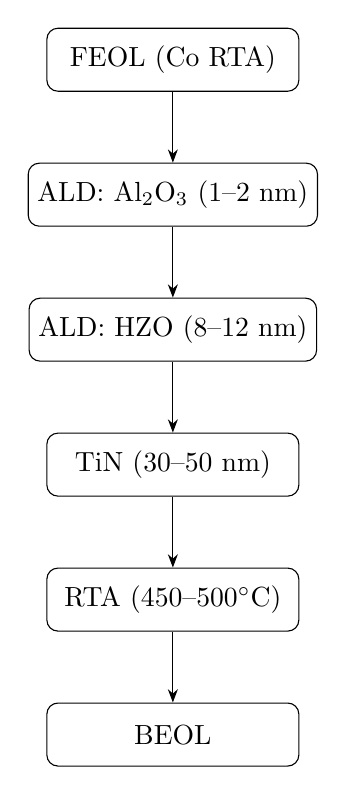
\begin{tikzpicture}[node distance=0.9cm,
  box/.style={draw, rectangle, rounded corners, minimum width=3.2cm, minimum height=0.8cm}]
\node[box] (a) {FEOL (Co RTA)};
\node[box, below=of a] (b) {ALD: Al\(_2\)O\(_3\) (1--2 nm)};
\node[box, below=of b] (c) {ALD: HZO (8--12 nm)};
\node[box, below=of c] (d) {TiN (30--50 nm)};
\node[box, below=of d] (e) {RTA (450--500$^\circ$C)};
\node[box, below=of e] (f) {BEOL};
\draw[->] (a)--(b);
\draw[->] (b)--(c);
\draw[->] (c)--(d);
\draw[->] (d)--(e);
\draw[->] (e)--(f);
\end{tikzpicture}
\caption{Process flow of FeFET integration.}
\label{fig:proc_flow}
\end{figure}

\subsection{Cross Section}
\begin{figure}[t]
\centering
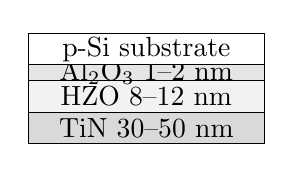
\begin{tikzpicture}
\draw[fill=gray!30] (0,0) rectangle (3,0.4) node[midway]{TiN 30--50 nm};
\draw[fill=gray!10] (0,0.4) rectangle (3,0.8) node[midway]{HZO 8--12 nm};
\draw[fill=gray!20] (0,0.8) rectangle (3,1.0) node[midway]{Al\(_2\)O\(_3\) 1--2 nm};
\draw[fill=white] (0,1.0) rectangle (3,1.4) node[midway]{p-Si substrate};
\end{tikzpicture}
\caption{Cross section of HZO/Al\(_2\)O\(_3\)/TiN stack.}
\label{fig:cross_section}
\end{figure}

\section{Devices and Methods}
Test structures include FeCAPs (flat/comb) and \SI{100}{\micro m}\(\times\)\SI{100}{\micro m} FeFET cells.
Programming used \(\pm\)2.3–\SI{2.7}{V}, \SI{1}{–}\SI{50}{\micro s} pulses.
Keysight B1500A and a manual prober were used.\\
\textbf{Protocols:}
TZDB: DC ramp \(\approx \SI{0.1}{V/s}\) at RT–\SI{125}{\celsius}.
TDDB: constant–voltage stress at 2.3/2.5/2.7 V, \SI{85}{\celsius} and \SI{125}{\celsius}; Weibull fitting.
Endurance: \(\pm\SI{2.5}{V}\), \SI{10}{\micro s}, \SI{10}{kHz} up to \(10^{5}\) cycles.
Retention: \SI{25}{\celsius}, \SI{85}{\celsius}, \SI{125}{\celsius}, with Arrhenius extrapolation.

\section{Results}

\subsection{TZDB}
Breakdown statistics indicate early–failure tails due to defects (Fig.~\ref{fig:tzdb}).
\begin{figure}[t]
\centering
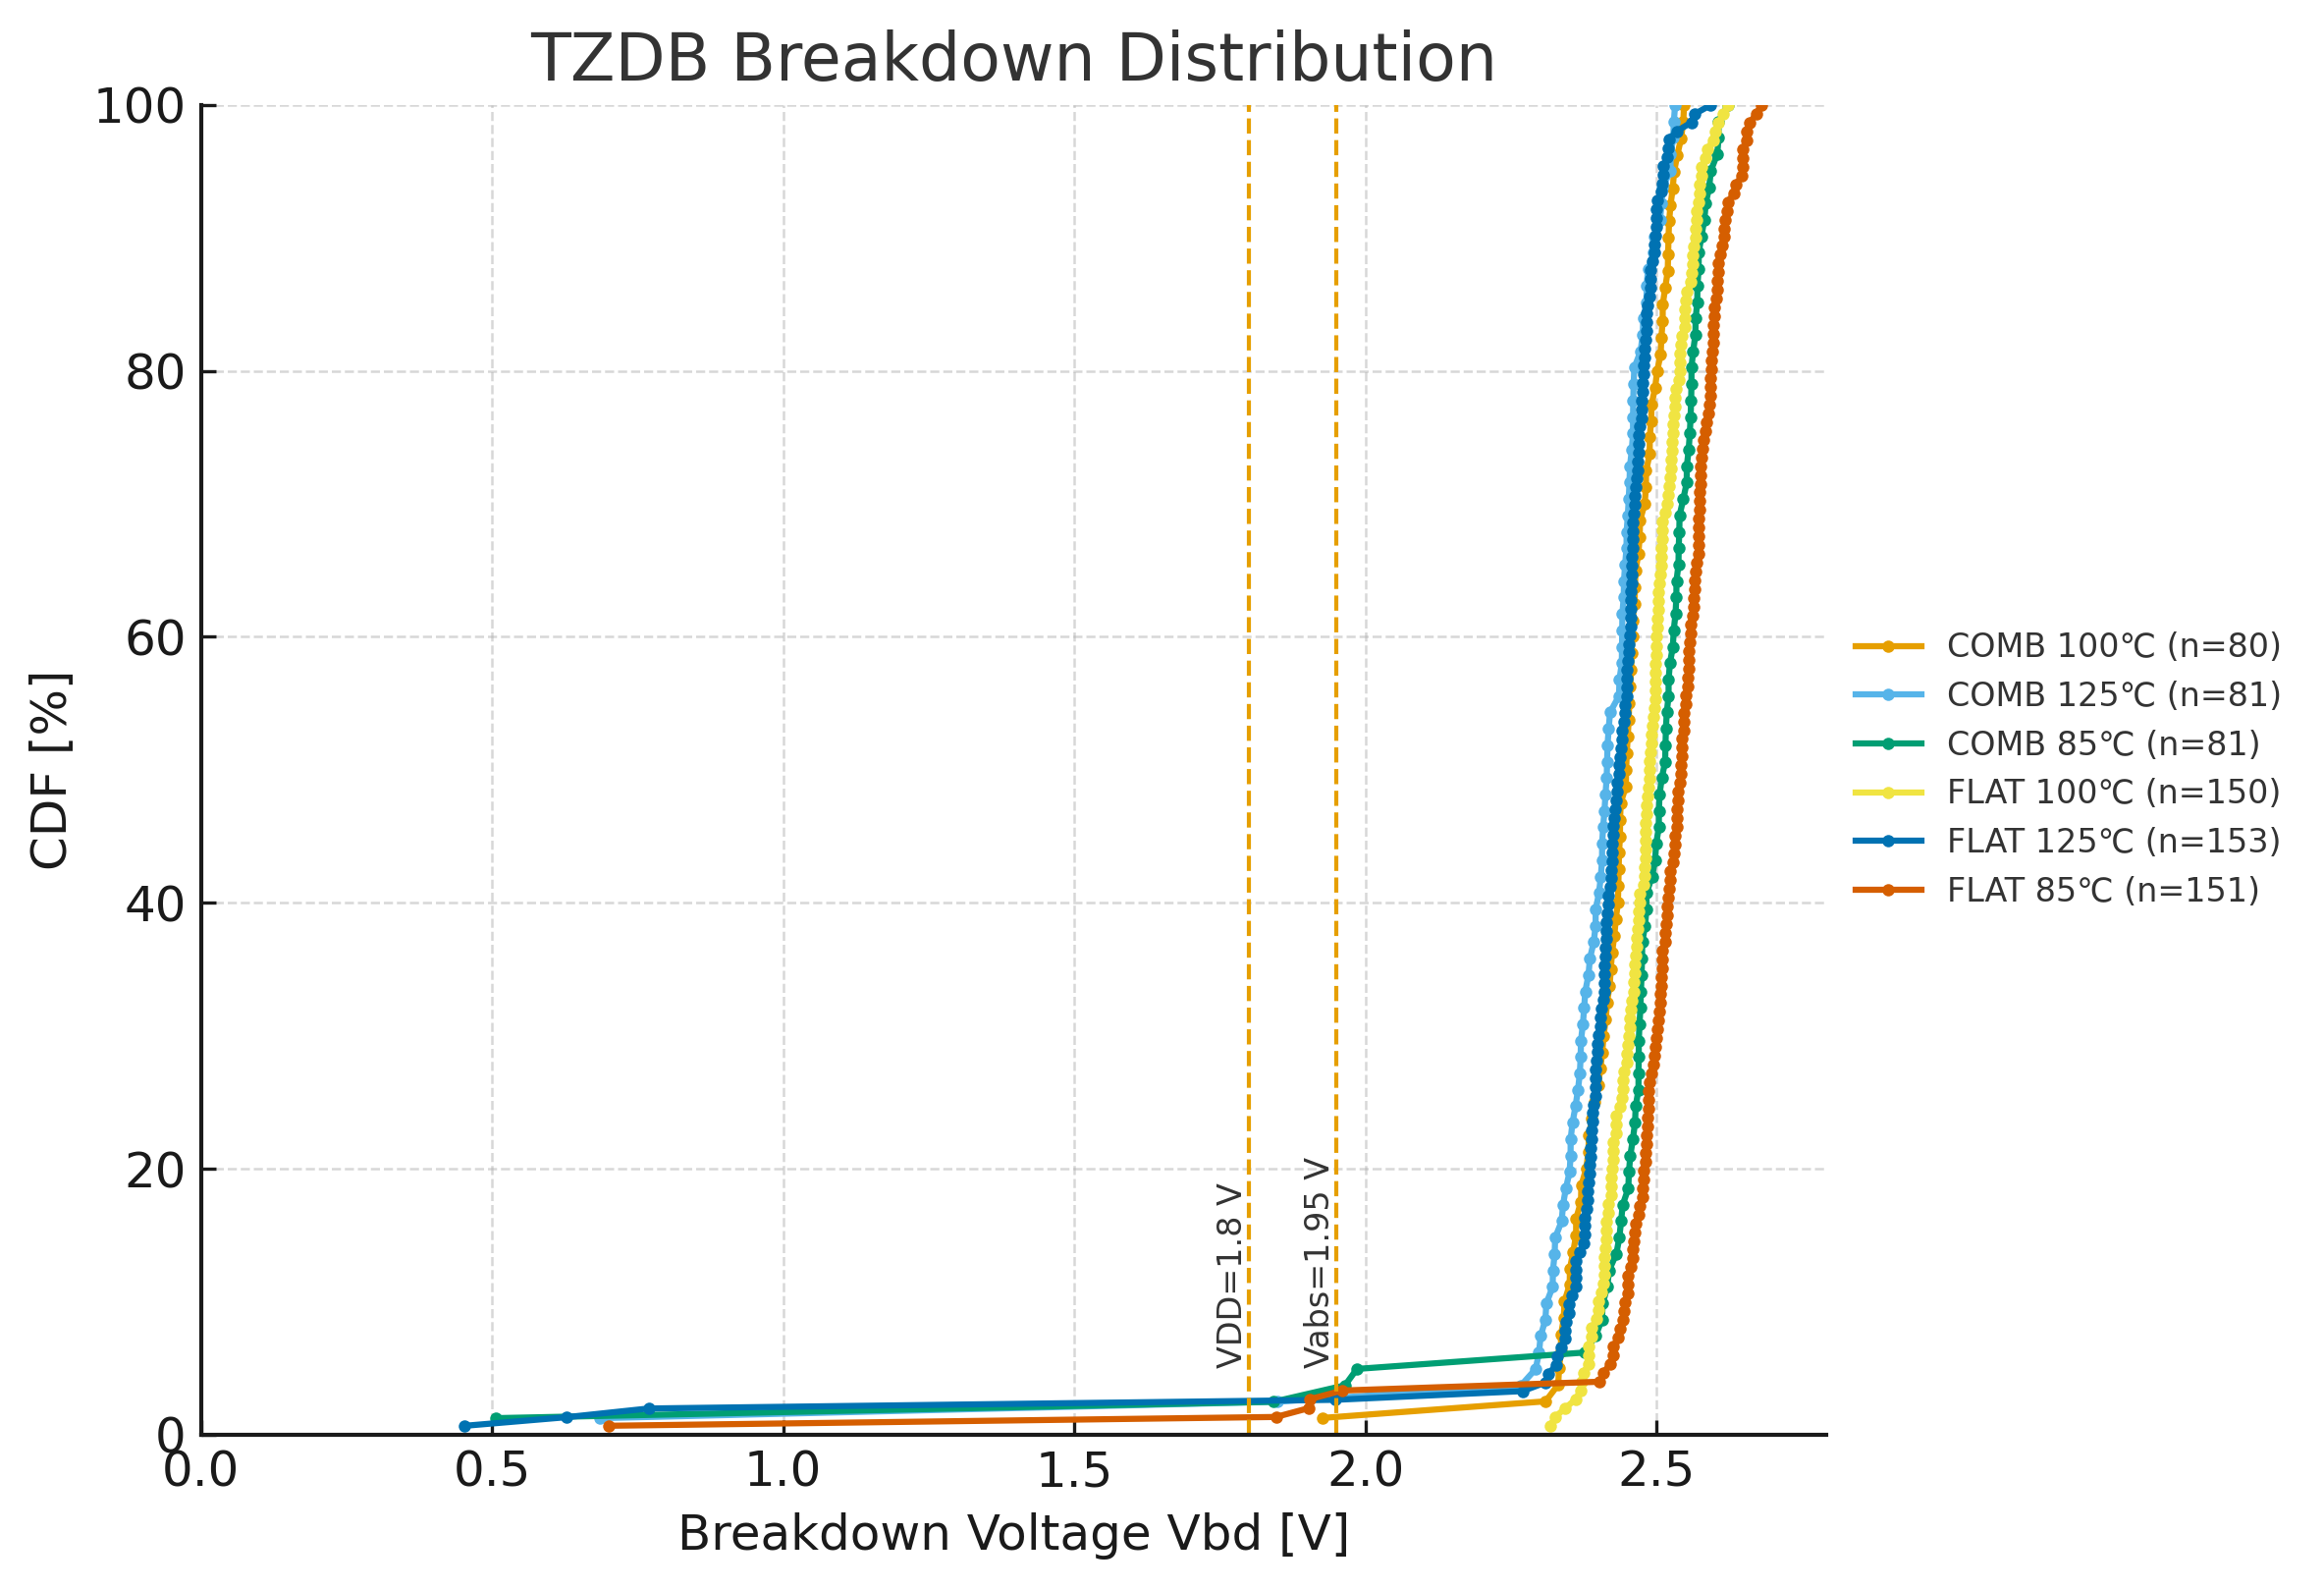
\includegraphics[width=\linewidth]{figures/fig3_tzdb.png}
\caption{TZDB distributions of FeCAPs.}
\label{fig:tzdb}
\end{figure}

\subsection{TDDB (Weibull/Arrhenius)}
Weibull plots yield \(\beta \approx 1.3\).
Arrhenius analysis gives activation energies consistent with oxygen–vacancy diffusion:
\(E_a \approx \SI{0.78}{eV}\) @ 2.3 V, \(\SI{0.84}{eV}\) @ 2.5 V, \(\SI{0.88}{eV}\) @ 2.7 V.

\begin{figure}[t]
\centering
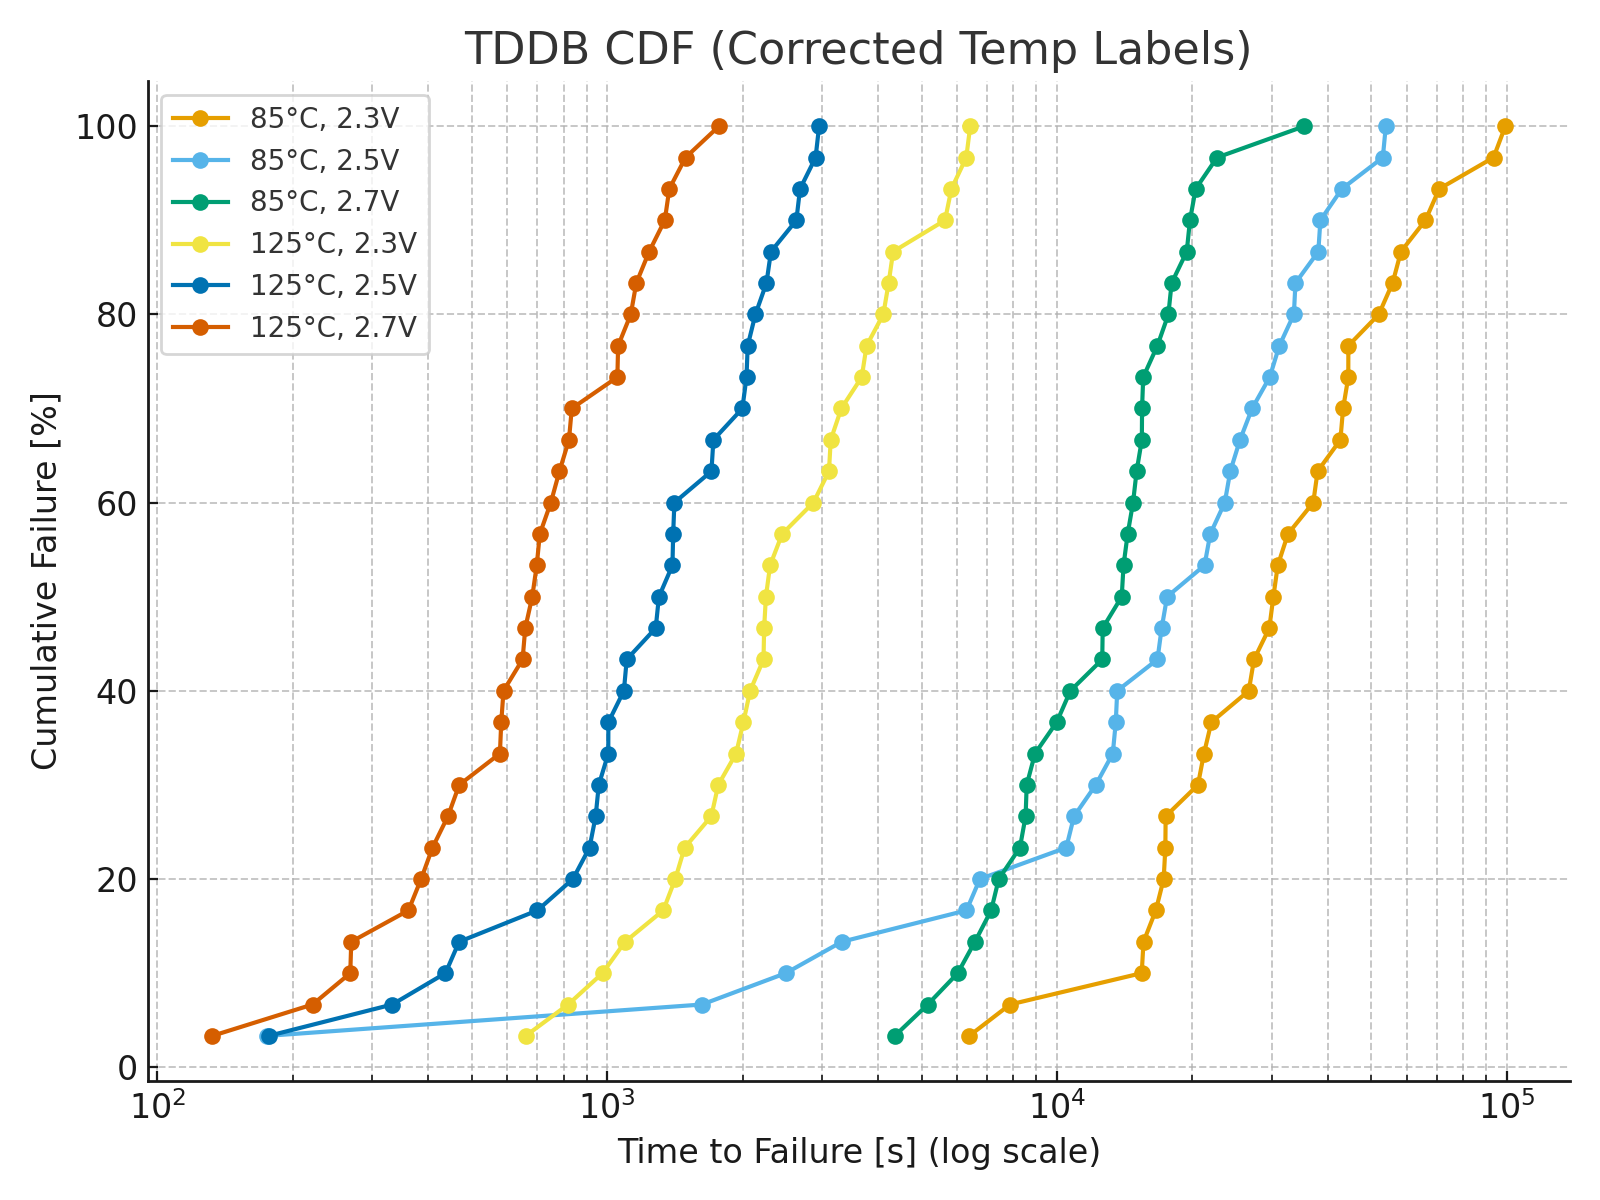
\includegraphics[width=\linewidth]{figures/fig4_tddb_cdf.png}
\caption{TDDB CDF under all stress conditions.}
\label{fig:tddb_cdf}
\end{figure}

\begin{figure}[t]
\centering
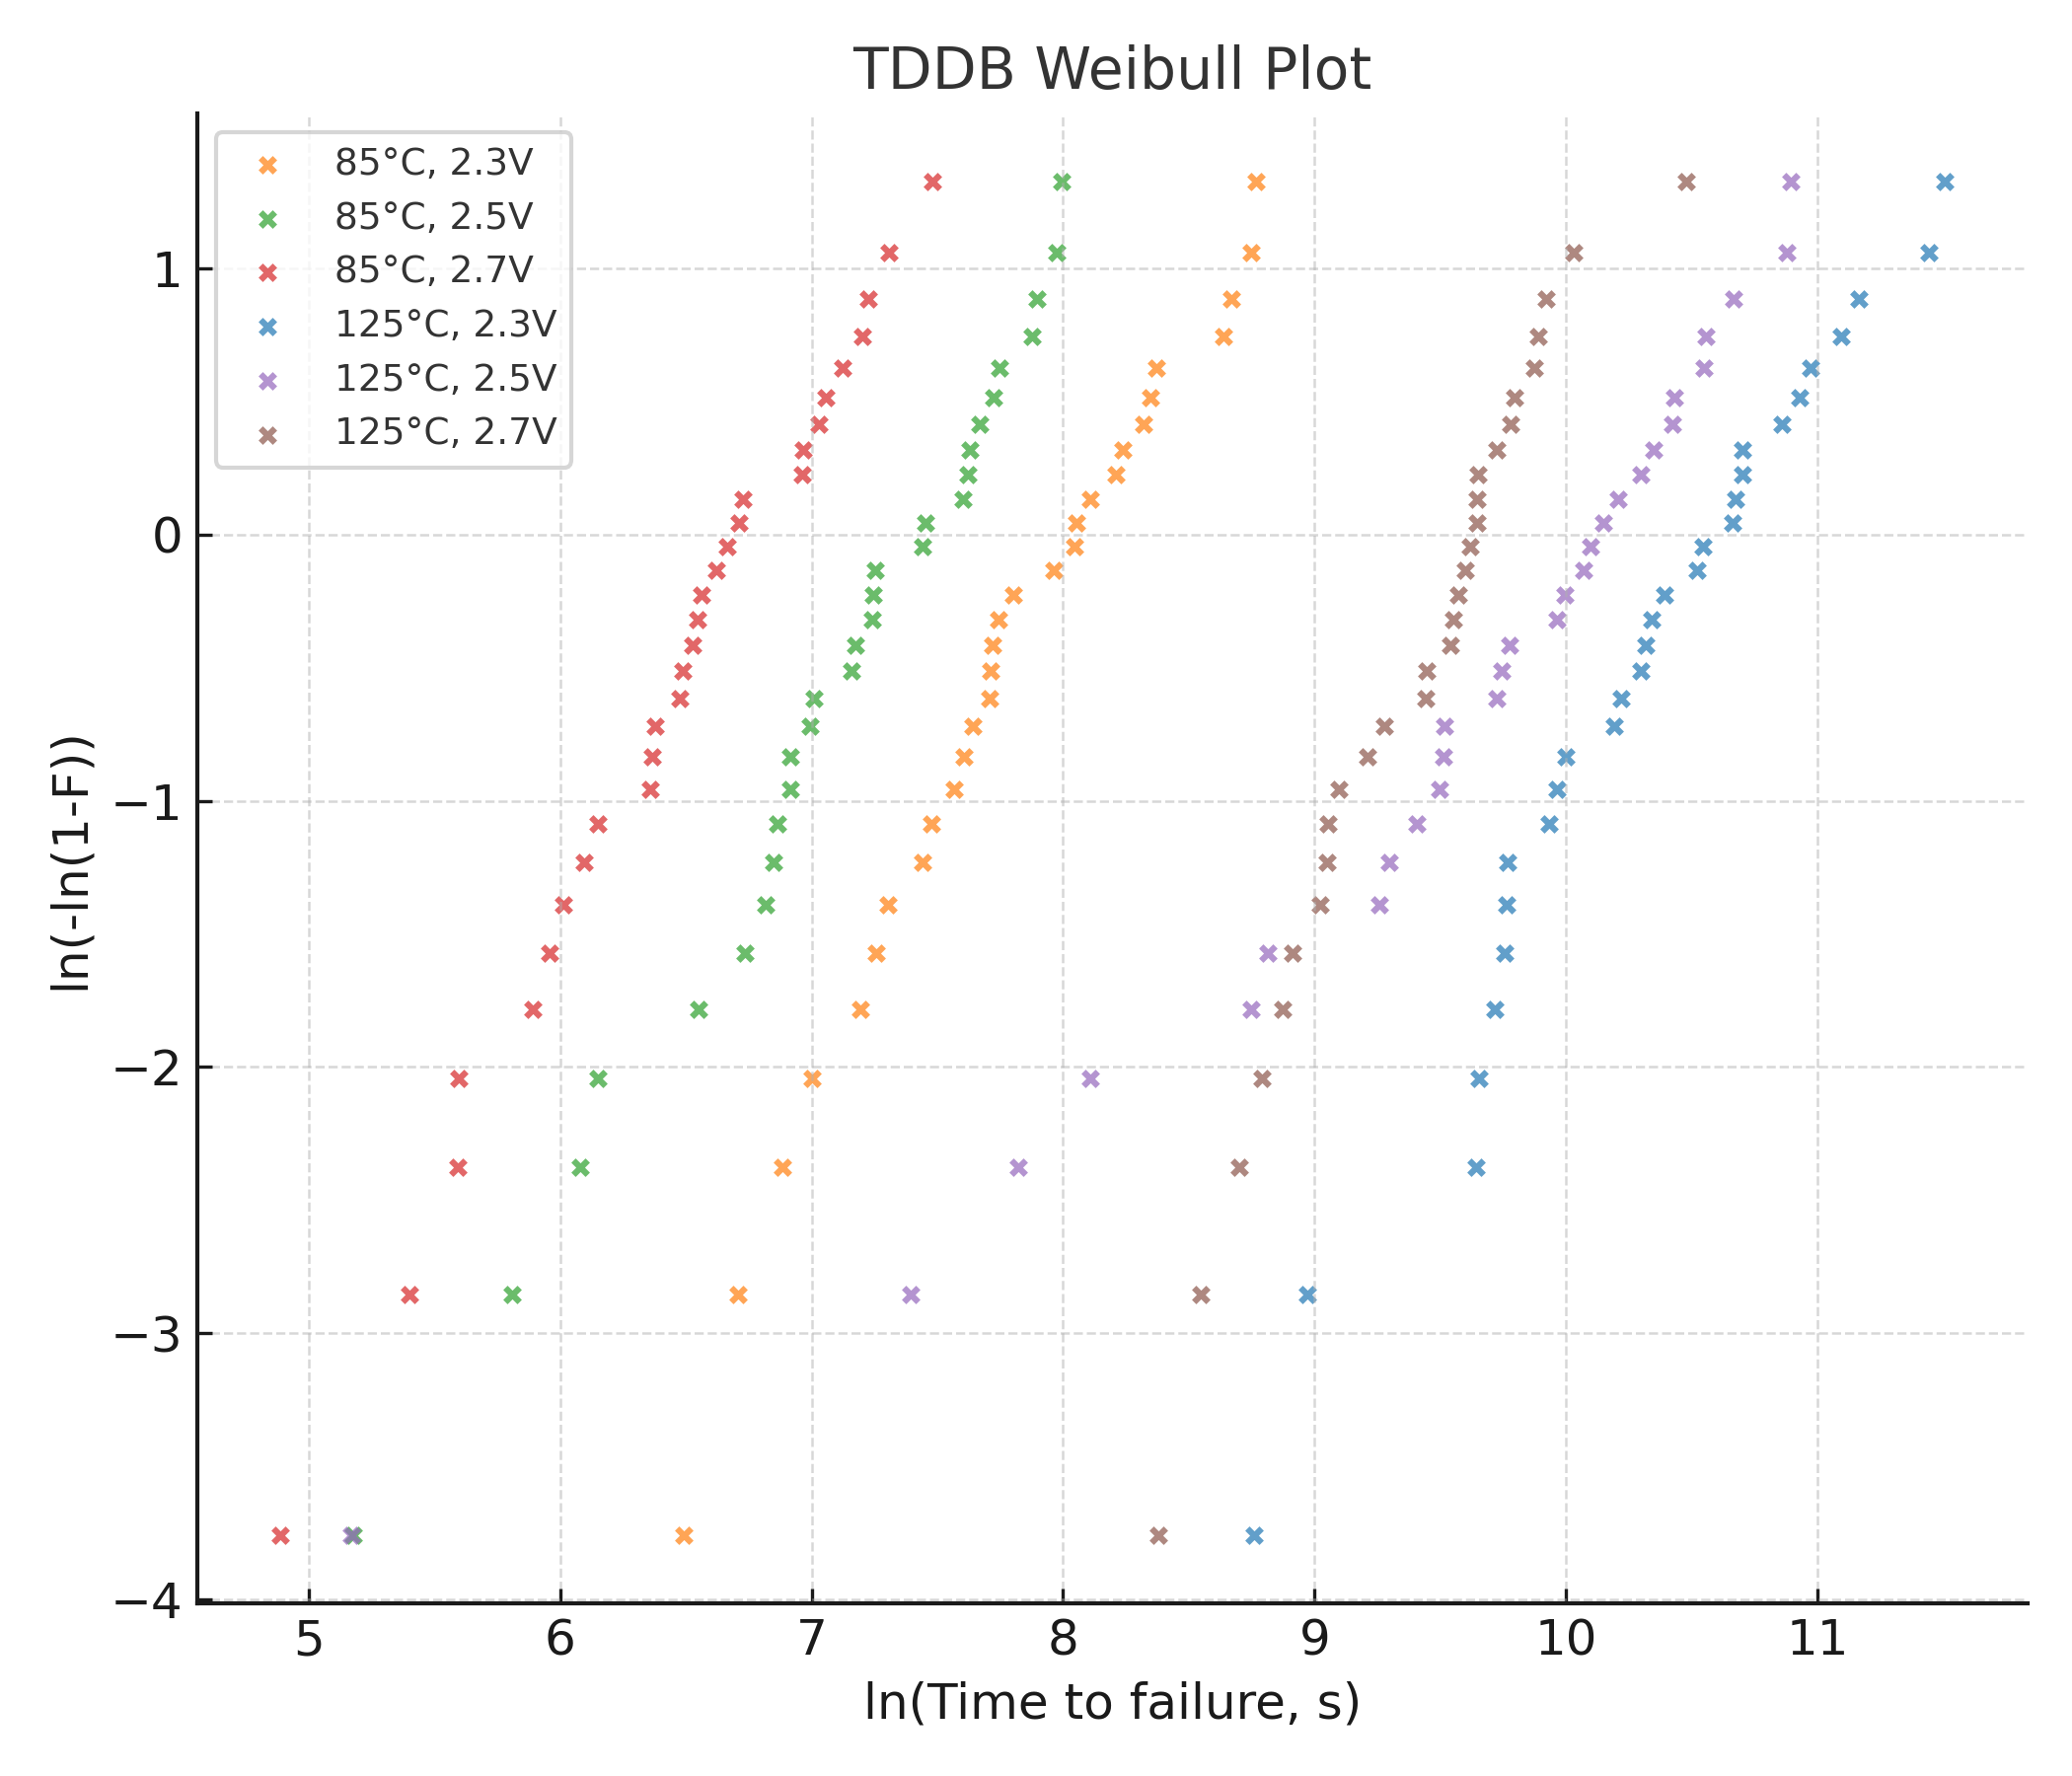
\includegraphics[width=\linewidth]{figures/fig4_tddb_weibull.png}
\caption{TDDB Weibull plots with fitted lines (\(\beta,\eta\)).}
\label{fig:tddb_weibull}
\end{figure}

\begin{table}[t]
\centering
\caption{Extracted TDDB scales \(\eta\) (representative).}
\begin{tabular}{@{}ccc@{}}
\toprule
Stress & Temp & \(\eta\) [s] \\
\midrule
2.3 V & \SI{85}{\celsius}  & \(2.7\times 10^{3}\) \\
2.3 V & \SI{125}{\celsius} & \(5.1\times 10^{4}\) \\
2.5 V & \SI{85}{\celsius}  & \(1.5\times 10^{3}\) \\
2.5 V & \SI{125}{\celsius} & \(2.8\times 10^{4}\) \\
2.7 V & \SI{85}{\celsius}  & \(8.2\times 10^{2}\) \\
2.7 V & \SI{125}{\celsius} & \(1.5\times 10^{4}\) \\
\bottomrule
\end{tabular}
\end{table}

\subsection{Endurance}
Up to \(10^{5}\) cycles verified; the window shrinks 20–30\%.
A compact fit is \(\Delta V_\mathrm{th}(N)=1.12-0.05\log_{10}N\).
\begin{figure}[t]
\centering
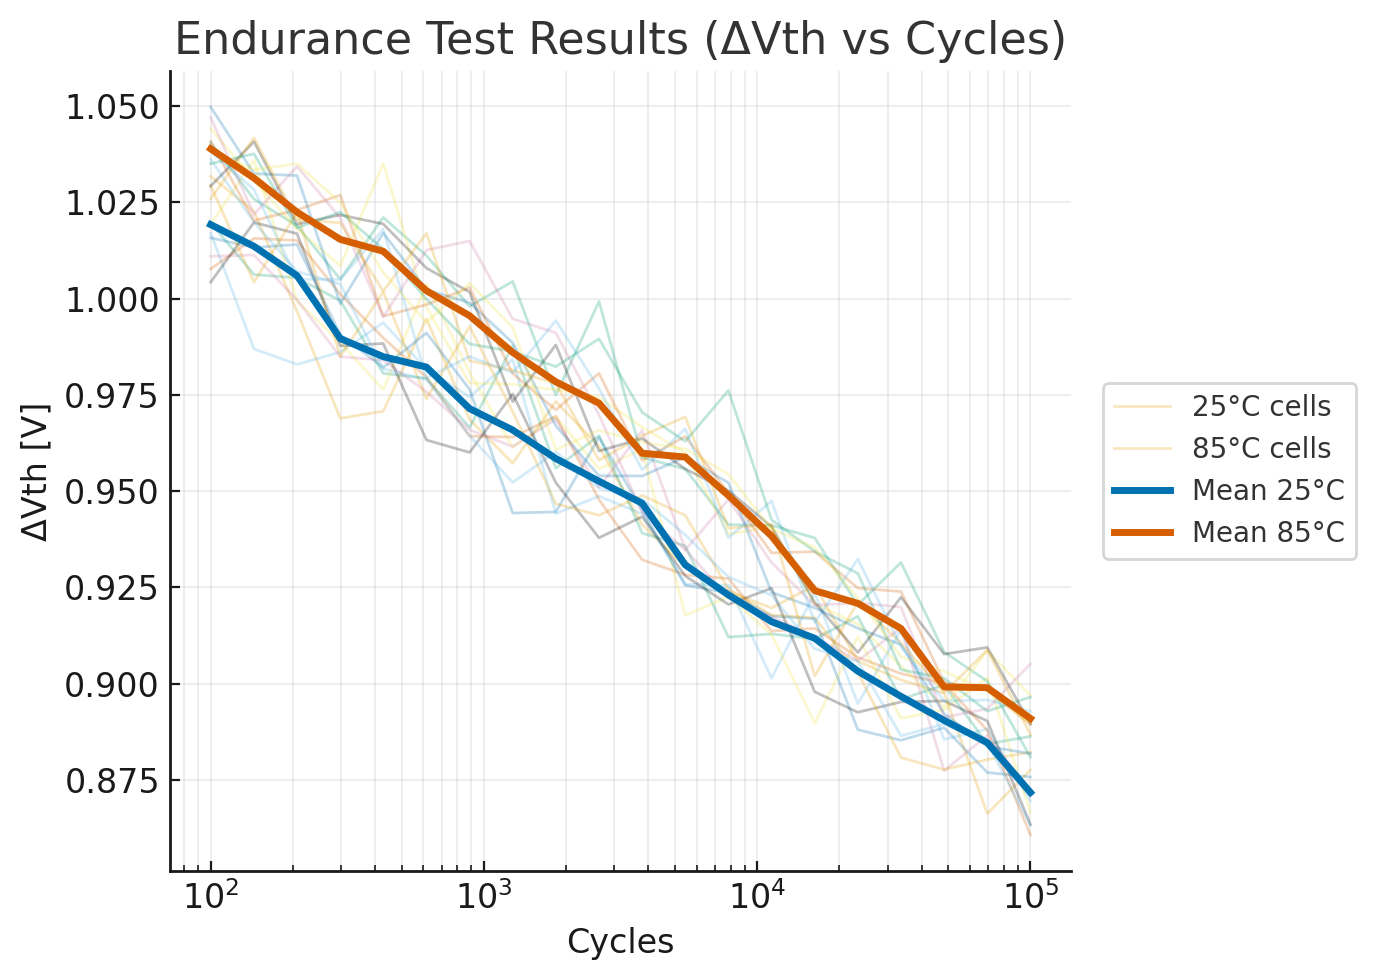
\includegraphics[width=\linewidth]{figures/fig5_endurance.png}
\caption{Endurance characteristics (\(\Delta V_{\mathrm{th}}\) vs. cycles).}
\label{fig:endurance}
\end{figure}

\subsection{Retention}
Arrhenius extrapolation with \(E_a \approx \SI{1.1}{eV}\) predicts:
\(> 10^{2}\) years @ \SI{25}{\celsius},
\(> 10\) years @ \SI{85}{\celsius},
and only months @ \SI{150}{\celsius}.
\begin{figure}[t]
\centering
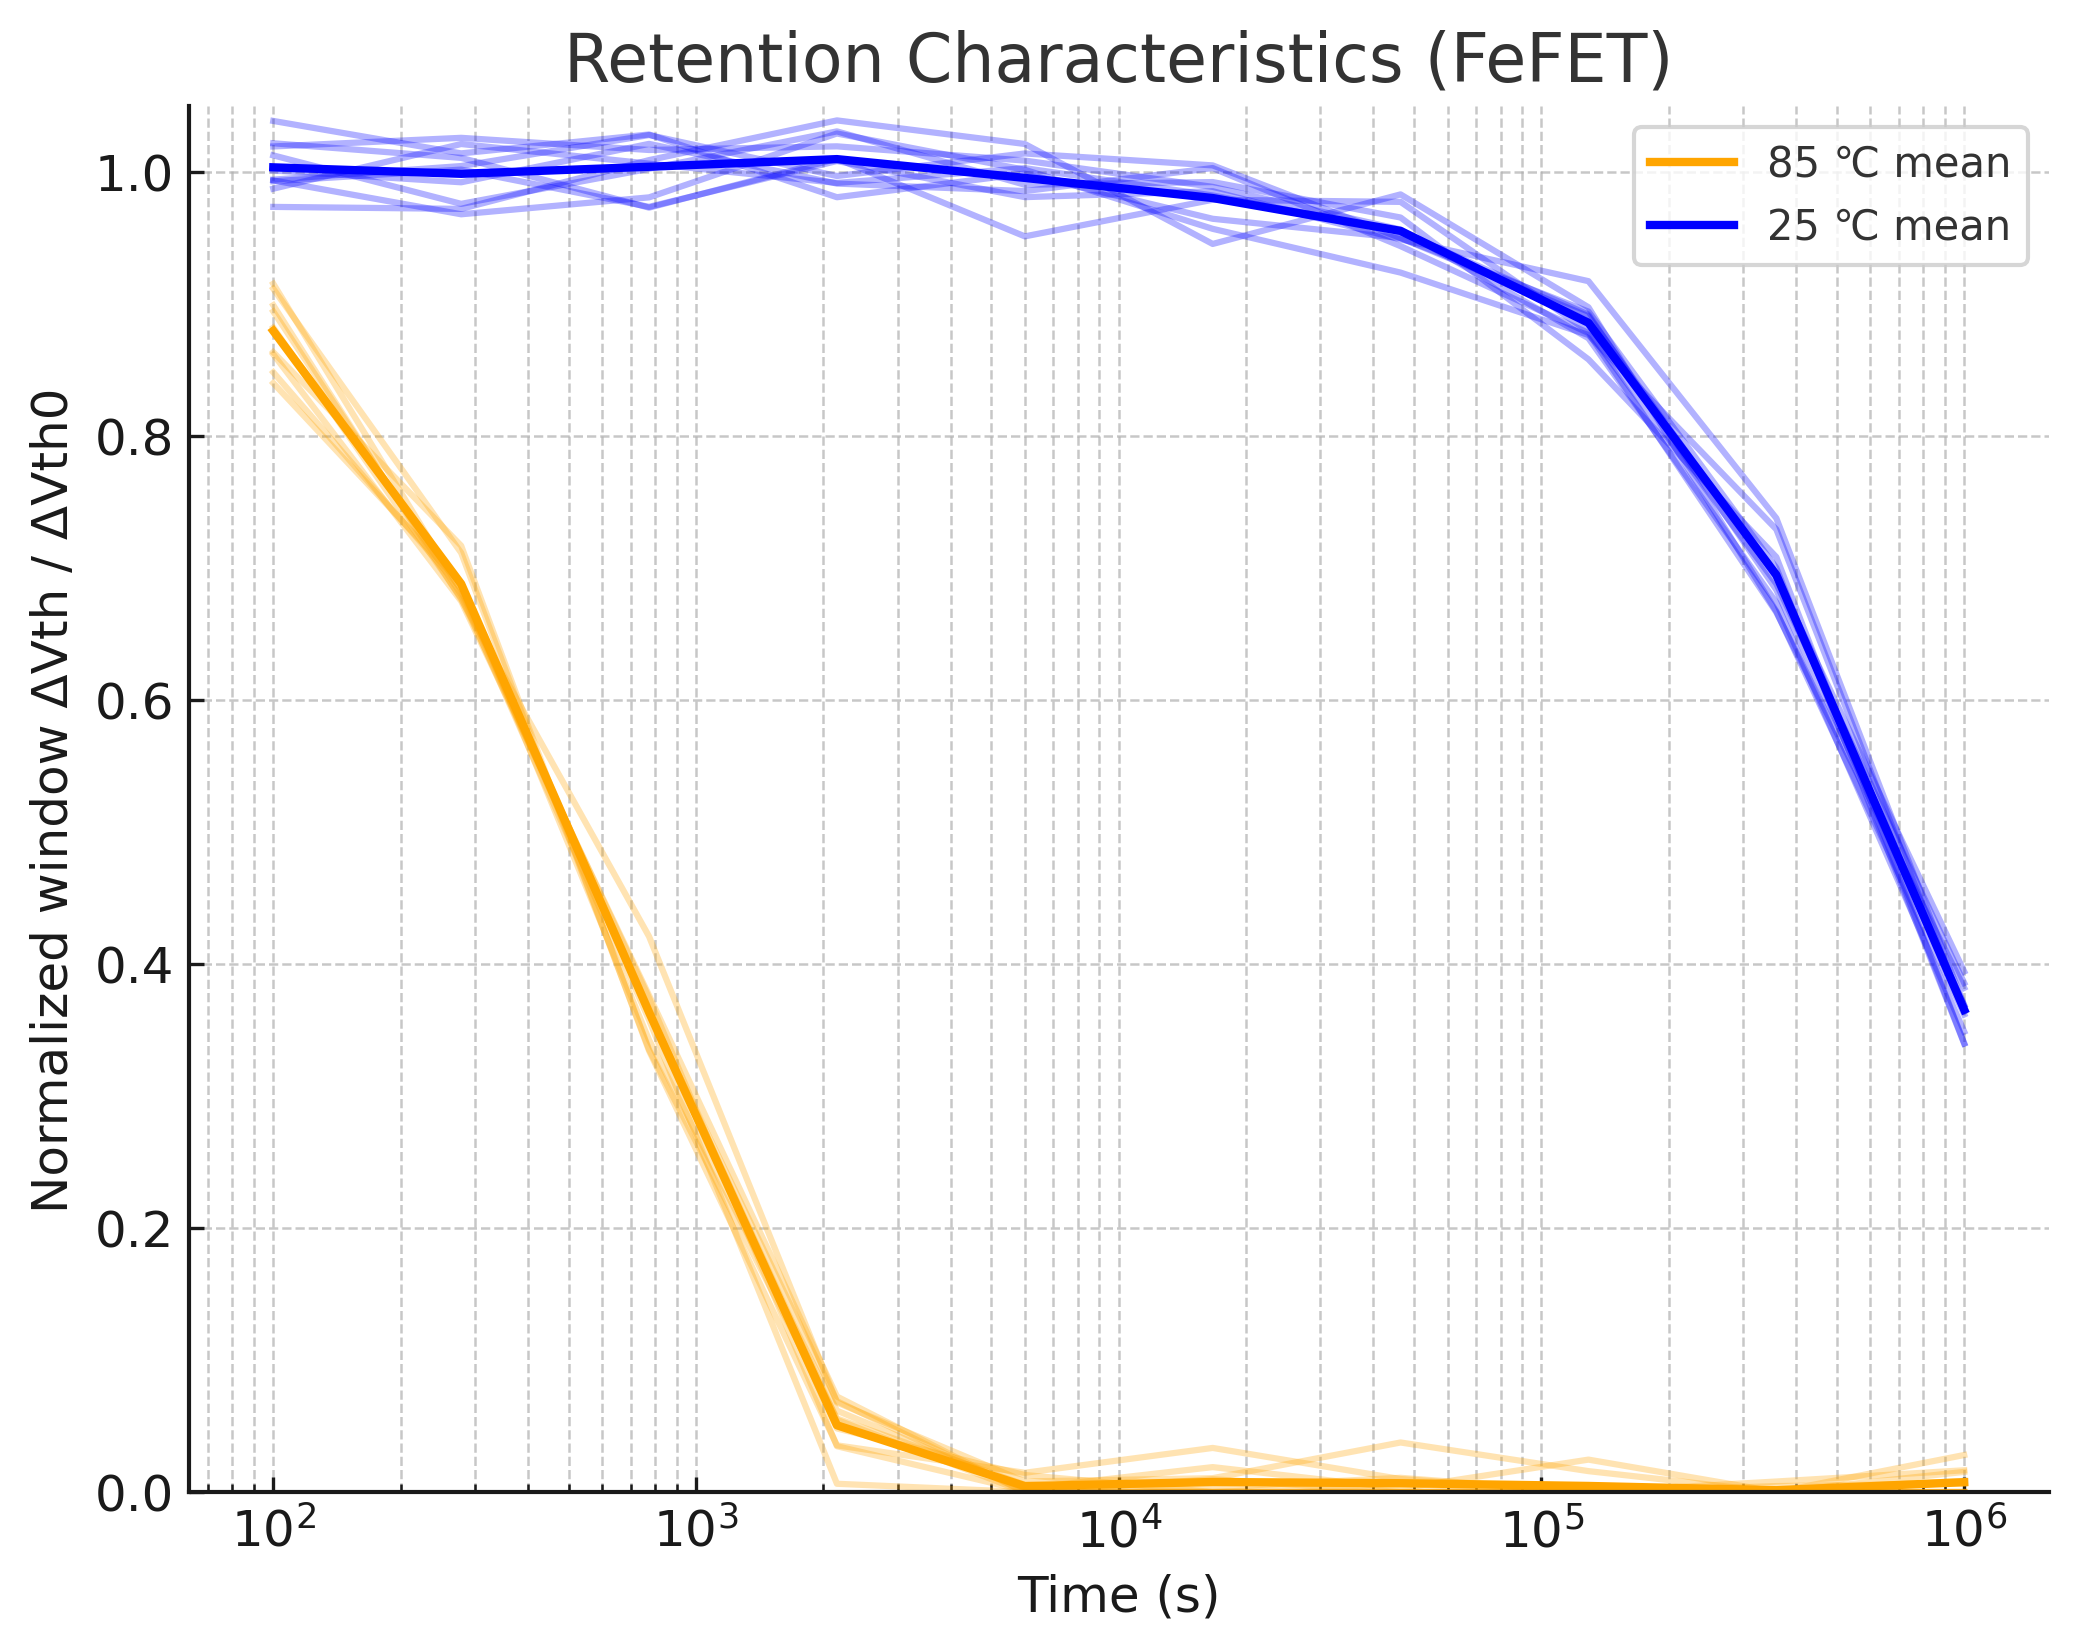
\includegraphics[width=\linewidth]{figures/fig6_retention.png}
\caption{Retention characteristics and Arrhenius extrapolation.}
\label{fig:retention}
\end{figure}

\section{System Architecture (SRAM + FeFET)}
\begin{figure}[t]
\centering
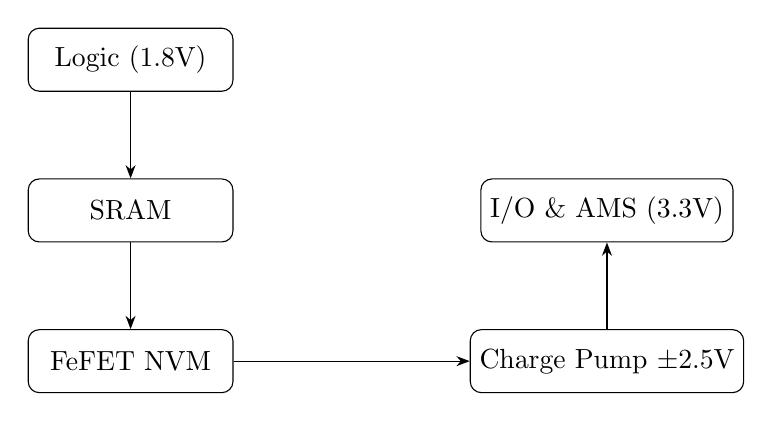
\begin{tikzpicture}[node distance=1.1cm,
  blk/.style={draw, rectangle, rounded corners, minimum width=2.6cm, minimum height=0.8cm}]
\node[blk] (logic) {Logic (1.8V)};
\node[blk, below=of logic] (sram) {SRAM};
\node[blk, below=of sram] (fefet) {FeFET NVM};
\node[blk, right=3.0cm of fefet] (pump) {Charge Pump $\pm$2.5V};
\node[blk, above=of pump] (io) {I/O \& AMS (3.3V)};
\draw[->] (logic)--(sram);
\draw[->] (sram)--(fefet);
\draw[->] (fefet)--(pump);
\draw[->] (pump)--(io);
\end{tikzpicture}
\caption{System architecture with SRAM + FeFET backup.}
\label{fig:system}
\end{figure}

\begin{figure}[t]
\centering
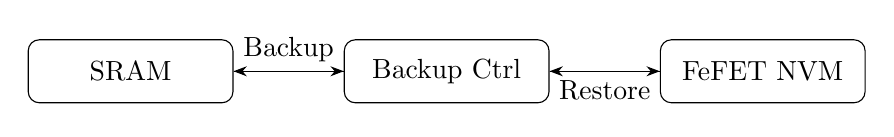
\begin{tikzpicture}[node distance=1.4cm,
  blk/.style={draw, rectangle, rounded corners, minimum width=2.6cm, minimum height=0.8cm}]
\node[blk] (sram2) {SRAM};
\node[blk, right=of sram2] (ctrl) {Backup Ctrl};
\node[blk, right=of ctrl] (nvm) {FeFET NVM};
\draw[->] (sram2)--(ctrl) node[midway,above]{Backup};
\draw[->] (ctrl)--(nvm);
\draw[->] (nvm)--(ctrl) node[midway,below]{Restore};
\draw[->] (ctrl)--(sram2);
\end{tikzpicture}
\caption{Backup/restore flow between SRAM and FeFET.}
\label{fig:backup}
\end{figure}

\section{Discussion}
The HZO/Al\(_2\)O\(_3\)/TiN stack provides sufficient reliability for industrial/consumer NVM.
For high–temperature automotive, improvements are required: IL optimization, crystallinity control, refresh/rewrite, and ECC.

\section{Conclusion}
We realized an FeFET module on \SI{0.18}{\micro m} CMOS with one extra mask and one ALD tool.
Devices exhibit \(>\!10^{5}\) cycles and \(>\!10\) years retention at \SI{85}{\celsius}.
The method extends mature–node lifetime and enables cost–effective embedded NVM for automotive/industrial/IoT.

\section*{Acknowledgment}
The author thanks collaborators for helpful discussions.

% ===== References =====
\begin{thebibliography}{99}
\bibitem{Boscke2011} T.~Böscke \emph{et al.}, Appl. Phys. Lett., vol.~99, p.~102903, 2011.
\bibitem{Mueller2012} J.~Müller \emph{et al.}, Appl. Phys. Lett., vol.~99, p.~112901, 2012.
\bibitem{Mikolajick2019} T.~Mikolajick \emph{et al.}, J. Appl. Phys., vol.~125, p.~204103, 2019.
\bibitem{Mueller2015} J.~Müller \emph{et al.}, IEEE Trans. Electron Devices, vol.~62, no.~12, pp.~4158--4166, 2015.
\bibitem{Park2020} J.~Park \emph{et al.}, IEEE Electron Device Lett., vol.~41, no.~5, pp.~711--714, 2020.
\bibitem{Nakamura2003} H.~Nakamura \emph{et al.}, IEEE Trans. Device Mater. Rel., vol.~3, no.~4, pp.~132--136, 2003.
\bibitem{Yamazaki2018} K.~Yamazaki \emph{et al.}, Jpn. J. Appl. Phys., vol.~57, 04FB07, 2018.
\end{thebibliography}

% ===== Biography =====
\section*{Biography}
\noindent
\textbf{Shinichi Samizo} has over 25 years of experience in semiconductor process integration and actuator development.
After studying control theory and EM modeling, he joined Seiko Epson in 1997 and worked on \SI{0.35}{\micro m}--\SI{0.18}{\micro m} CMOS logic/memory/HV integration, DRAM, and LCD drivers.
Later he contributed to PZT actuator development and the PrecisionCore inkjet head.
He is currently an independent researcher, publishing educational materials via the ``Project Design Hub''.
\end{document}
